% Regression test project.
% Each section lines up with a part of dev/regression/checklist.md.
% If a section doesn't look like its comment says, that's a regression.
\documentclass{article}
\usepackage{graphicx}
\usepackage{hyperref}

\title{Regression Test Project}
\author{LaTeX Collaborative Editor}
\date{1 January 2026}

\begin{document}

\maketitle

% Expect: a title, an author line, and the date 1 January 2026.

\section{Text}
% Expect: this section comes from chapters/text.tex through \input.

\subsection{Formatting}
This line has \textbf{bold}, \emph{emphasis}, \textit{italic}, \texttt{monospace}, and \underline{underlined} text.
Special characters: \& \% \$ \# \_ \{ \} and an en--dash and an em---dash.
Unicode: café, naïve, Zürich, and “curly quotes”.\footnote{Expect: this note shows. LaTeX.js puts it inline, not at the bottom.}

\subsection{Lists}
\begin{itemize}
  \item A bullet
  \item Another bullet
  \begin{itemize}
    \item A nested bullet
  \end{itemize}
\end{itemize}

\begin{enumerate}
  \item First
  \item Second
\end{enumerate}

\begin{description}
  \item[Term] Its description.
\end{description}

\subsection{Blocks}
\begin{quote}
A quote, indented on both sides.
\end{quote}

\begin{center}
Centered text.
\end{center}

\subsection{Links}
% Expect: the first three are links. Clicking the first two opens them in a new tab, and the
% preview itself stays put. Clicking the email link hands it to your mail app.
% The last two must show as text with no href, since the preview strips unsafe links.
\href{https://github.com/PrestonHager/LaTeXCollaborativeEditor}{The repository},
\url{https://example.com},
\href{mailto:someone@example.com}{an email link},
\href{javascript:alert(1)}{a javascript link},
and \href{data:text/html,hi}{a data link}.

\subsection{References}
\label{sec:refs}
This is section~\ref{sec:refs}.
% Expect: clicking the 4 in the next line scrolls the preview down to the Citations section.
Jump to section~\ref{sec:citations}.
% Expect: ?? as plain text, not a link, since the label doesn't exist.
A missing label: \ref{sec:does-not-exist}.

\subsection{Verbatim}
% Expect: the \verb text shows in monospace exactly as typed, backslashes and braces included.
% Expect: nothing from the comment block shows, and "Before" and "after" stay in one paragraph.
% Expect: the "Preview is approximate" list (the info button above the preview) doesn't mention \vspace or \addcontentsline,
% since both only appear inside verbatim-like text.
Inline code: \verb|\vspace{1em}| and \verb+\footnote{not a footnote}+.
Before \begin{comment}\addcontentsline{toc}{section}{Hidden}\end{comment} after.


\section{Math}
% Expect: every formula typeset with KaTeX, none shown as raw TeX.

Inline math like $e^{i\pi} + 1 = 0$ and $\sqrt{a^2 + b^2}$ sits in the line.

Display math:
\[
  \int_0^1 x^2 \, dx = \frac{1}{3}
\]

A sum, with limits above and below:
\[
  \sum_{k=1}^{n} k = \frac{n(n+1)}{2}
\]

Greek and symbols: $\alpha, \beta, \gamma, \infty, \leq, \neq, \rightarrow$.

% Expect: every symbol below in a serif math font, same size as the text around it.
% \neq, \ne, \notin and \not\equiv show a slash through the symbol, not a box or a stray mark (issue #82).
Symbols Computer Modern lacks: $\infty$, $a \neq b$, $a \ne b$, $x \notin A$, $a \not\equiv b$,
$\leq, \geq, \in, \forall, \exists, \partial, \nabla, \pm, \hbar, \ell, \emptyset, \approx, \equiv, \subseteq, \Rightarrow, \iff$.

A matrix: $\left( \begin{array}{cc} 1 & 0 \\ 0 & 1 \end{array} \right)$.


% A commented-out input must be skipped, not loaded or reported as missing.
% \input{chapters/does-not-exist}

\section{Figures}
% Expect: this section comes from chapters/figures.tex through \include.

\subsection{Images}
% Expect: the same four-color image, first full size with a caption under it.
% The image comes from figures/quadrants.png in the file tree.
\begin{figure}
  \centering
  
\includegraphics{figures/quadrants.png}
  \caption{A project image, full size.}
\end{figure}

\subsubsection{Image sizes}
% Expect: an image half as wide as the text column.

\includegraphics[width=0.5\textwidth]{figures/quadrants}

% Expect: an image 2cm wide (about 76px), with its height kept in proportion.

\includegraphics[width=2cm]{figures/quadrants}

% Expect: an image 1in tall (96px), with its width kept in proportion.

\includegraphics[height=1in]{figures/quadrants}

% Expect: an image stretched to 4cm wide and 1cm tall.

\includegraphics[width=4cm,height=1cm]{figures/quadrants}

% Expect: an image fitted inside 4cm by 1cm without stretching, so it is 1cm tall.

\includegraphics[width=4cm,height=1cm,keepaspectratio]{figures/quadrants}

% Expect: an image at half its natural size (48px by 32px).

\includegraphics[scale=0.5]{figures/quadrants}

\subsection{PDF and EPS figures}
% Expect: a bar chart (red, green and blue bars on axes, "PDF figure p1" at the top) at its
% natural size, 2in by 1.33in. It comes from page 1 of figures/chart.pdf, drawn with pdf.js.
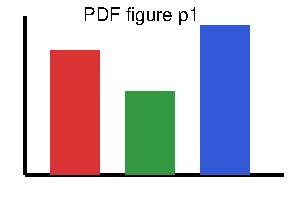
\includegraphics{figures/chart.pdf}

% Expect: page 2 of the same PDF, a blue diamond with "page 2" on it, 3cm wide.
\includegraphics[page=2,width=3cm]{figures/chart}

% Expect: only the right-hand blue bar of page 1, cut out with trim and clip, 1in tall.
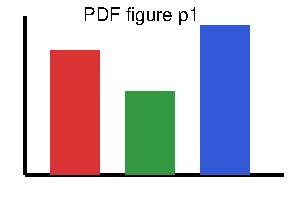
\includegraphics[trim=90bp 8bp 18bp 11bp,clip,height=1in]{figures/chart.pdf}

% Expect: a dashed box 2in by 1in (the file's %%BoundingBox) with the name figures/wave.eps
% and "EPS can't be previewed; convert it to PDF." in it. The ⓘ list says EPS figures show as boxes.
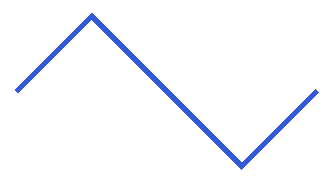
\includegraphics{figures/wave.eps}

% Expect: the same EPS box at half the column width, keeping its 2:1 shape.
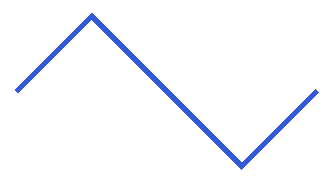
\includegraphics[width=0.5\textwidth]{figures/wave}

\subsection{Pictures}
% Expect: a box with a line across it and a circle in the middle.
% A picture compiles on the main thread instead of the worker, since LaTeX.js needs the real DOM to size it.
\setlength{\unitlength}{1mm}
\begin{picture}(40,20)
  \put(0,0){\framebox(40,20){}}
  \put(0,0){\line(2,1){40}}
  \put(20,10){\circle{8}}
\end{picture}


\section{Citations}
% Expect: [1] and [2] in the text, then a References list with both entries.
Knuth wrote the book on \TeX{} \cite{knuth}, and Lamport wrote one on \LaTeX{} \cite{lamport}.
Citing the same key again keeps its number \cite{knuth}.

\bibliographystyle{plain}
\bibliography{refs}

\end{document}
